% %%%%%%%%%%%%%%%%%%%%%%%%%%%%%%%%%%%%%%%%%%%%%%%%%%%%%%%%%
% | - Electrochemical OER Application
% %%%%%%%%%%%%%%%%%%%%%%%%%%%%%%%%%%%%%%%%%%%%%%%%%%%%%%%%%
%
% OER DFT modelling references:
%   * Man2011
% __|
% %%%%%%%%%%%%%%%%%%%%%%%%%%%%%%%%%%%%%%%%%%%%%%%%%%%%%%%%%



% %%%%%%%%%%%%%%%%%%%%%%%%%%%%%%%%%%%%%%%%%%%%%%%%%%%%%%%%%
% | - Short Intro EChem Section
%
% __|
% %%%%%%%%%%%%%%%%%%%%%%%%%%%%%%%%%%%%%%%%%%%%%%%%%%%%%%%%%
% | - PARAGRAPH BODY
%
% TODO In the previous sections make sure to highlight the alpha and rutile IrO3 phases explicitely so that this sentence makes sense here.
We next performed \latin{ab-initio} thermodynamic simulations to elucidate the electrochemical operational stability of \IrOx and the oxygen evolution reaction (OER) activity of various \IrOthree phases previously computed.
%
In particular, we have decided to compare the stability and activity of the most stable \IrOtwo and \IrOthree polymorphs (rutile and our newly discovered \aIrOthree phase), and the rutile-like \IrOthree polymorph.
%
In addition, we computed the OER activity of a delithiated form of a recently reported $\beta$-Li\textsubscript{x}IrO\textsubscript{3} (referred to here as \bIrOthree) structure, as it is a notable example of a well characterized experimental \IrOthree OER catalyst with exceptional activity.~\cite{Pearce2017,Pearce2019}
% __|
% %%%%%%%%%%%%%%%%%%%%%%%%%%%%%%%%%%%%%%%%%%%%%%%%%%%%%%%%%


% %%%%%%%%%%%%%%%%%%%%%%%%%%%%%%%%%%%%%%%%%%%%%%%%%%%%%%%%%
% | - Bulk Pourbaix Diagram
%
% Explain the Ir and IrO[4-] species
% QUESTION Use E or U for potential variable
% __|
% %%%%%%%%%%%%%%%%%%%%%%%%%%%%%%%%%%%%%%%%%%%%%%%%%%%%%%%%%
% | - PARAGRAPH BODY
%
The bulk Pourbaix diagram of the Ir-H2O system is shown in Figure~\ref{fig:bulk_pourbaix}.
%
The diagram was constructed by considering the equilibrium between with the following species: Ir, \rIrOtwo, \aIrOthree,  \rIrOthree, \bIrOthree, and an aqueous dissolved \ce{IrO[4-]} species.
%
We utilized a free energy correction scheme to reproduce the experimental free energy of \IrOtwo relative the Ir reference state, see the Supplementary Information for further details.
%
While Ir and \rIrOtwo are most stable at low bias, \aIrOthree becomes the thermodynamically dominant phase under the relevant conditions for the OER (potentials around \mytilde1.23 V vs. RHE and an acidic environment)
%
% I want to be careful about how I talk about the metastable structures in the bulk Pourbaix, they strictly speaking shouldn't be there at all
The stability regions of the metastable \rIrOthree and \bIrOthree phases (In the absence of any other \IrOthree polymorph) are indicated by unfilled solid lines, and show that these phases also have a large stability window relative to \IrOtwo and the Ir ion.
%
There are twenty one unique \IrOthree polymorphs discovered in our search which have a region of stability in the bulk Pourbaix plot, in the pH window of zero to sixteen.
%
% TODO Create energy table for main bulk systems in SI
% The similar formation energies (see Table \ref{table:oer_table}) for all three \IrOthree species suggest some or all of these \IrOthree phases may be present and are stable under OER conditions.
% __|
% %%%%%%%%%%%%%%%%%%%%%%%%%%%%%%%%%%%%%%%%%%%%%%%%%%%%%%%%%


% =========================================================
% FIGURE ==================================================
% =========================================================
% | - Figure | Bulk Pourbaix Diagram
\begin{figure*}[!htb]
\centering
\makebox[\textwidth][c]{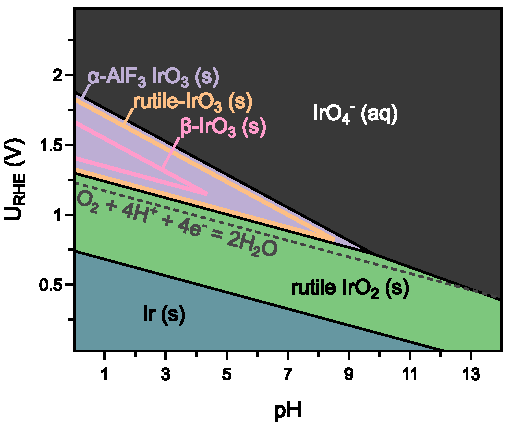
\includegraphics{02_figures/oer_activity_stability/bulk_pourbaix.pdf}}
\caption{\label{fig:bulk_pourbaix}
%
Revised bulk Pourbaix diagram of the Ir-H$_2$O system as a function of applied potential and pH.
%
The diagram was constructed with Ir(s) (blue), \rIrOtwo (green), various \IrOthree polymorphs and a dissolved
a dissolved \ce{IrO\textsubscript{4}[-]} ion species (dark grey).
%
The stabiliy regions corresponding to the metastable \rIrOthree and \bIrOthree polymorphs, in the absence of any competing \IrOthree phase, are displayed as yellow and pink lines, respectively. 
%
The thermodynamic onset of OER (water equilibrium at 1.23 V vs. RHE) is also shown.
%
% The most stable system studied (see Table XX in SI for a full list) are Ir-metal Ir(s) (blue), a \rIrOtwo (green), and a dissolved \ce{IrO4[4-]} (grey).
%
% These are compared to the \ce{IrO_3} polymorphs, \aIrOthree (purple), \rIrOthree (orange), and \bIrOthree (pink).
}
\end{figure*}
% __| =====================================================
% =========================================================


% %%%%%%%%%%%%%%%%%%%%%%%%%%%%%%%%%%%%%%%%%%%%%%%%%%%%%%%%%
% | - Introduction to OER Results
% 
% __|
% %%%%%%%%%%%%%%%%%%%%%%%%%%%%%%%%%%%%%%%%%%%%%%%%%%%%%%%%%
% | - PARAGRAPH BODY
%
The results of the electrochemical activity and surface stability analysis are summarized in Figure~\ref{fig:oer_volcano}.
%
There, we report the surface energy Pourbaix plots and OER activity for various surface facets at select coverages (*OH, *O, and bare) of the four \IrOx polymorphs from \ref{fig:bulk_pourbaix}.
%
The surface stability Pourbaix plots inform which surface facets and surface coverage species are thermodynamically preferred under OER conditions.
%
This analyis, allows us to consider both the stability and activity of particular surface terminations.
%
% TODO Insert XRD simulation into SI and reference here
For each polymorph, surface facets were selected by considering the highest intensity x-ray diffraction peaks from simulated powder-diffraction plots~\cite{Momma2011} (see Figure \ref{fig:xrd_patterns}),
as well as manually selecting high symmetry cleavage planes.
% __|
% %%%%%%%%%%%%%%%%%%%%%%%%%%%%%%%%%%%%%%%%%%%%%%%%%%%%%%%%%


% %%%%%%%%%%%%%%%%%%%%%%%%%%%%%%%%%%%%%%%%%%%%%%%%%%%%%%%%%
% | - Surface Energy Pourbaix Analysis
%
% __|
% %%%%%%%%%%%%%%%%%%%%%%%%%%%%%%%%%%%%%%%%%%%%%%%%%%%%%%%%%
% | - PARAGRAPH BODY
%
Figure~\ref{fig:oer_volcano}a reports the surface energy Pourbaix plots as a function of applied potential (at pH\num{=0}) for the four \IrOx crystals of interest.
%
The bulk phase limits of stability from Figure~\ref{fig:bulk_pourbaix} are included at the bottom of each subplot.
%
For each facet we computed the surface free energy for three coverages, bare, *OH, and *O.
%
At modest overpotentials ($\eta$ \mytilde\num{0.3} or equivalently potentials of \mytilde\num{1.5} V vs. RHE) the convex hull is populated solely by oxygen terminated surfaces.
%
% COMBAK, Revise "mainly" if we include some different coverages
Consequently, we consider mainly oxygen terminated surfaces for the OER analysis.
%
These results are comparable to previous studies on the electrochemical stability of \IrOtwo surfaces~\cite{Nattino2019}, but without considering highly reconstructed facets such as (101).
% __|
% %%%%%%%%%%%%%%%%%%%%%%%%%%%%%%%%%%%%%%%%%%%%%%%%%%%%%%%%%


% =========================================================
% FIGURE ==================================================
% =========================================================
% | - Figure | OER Volcano/Surface Pourbaix
\begin{figure*}
\centering
\makebox[\textwidth][c]{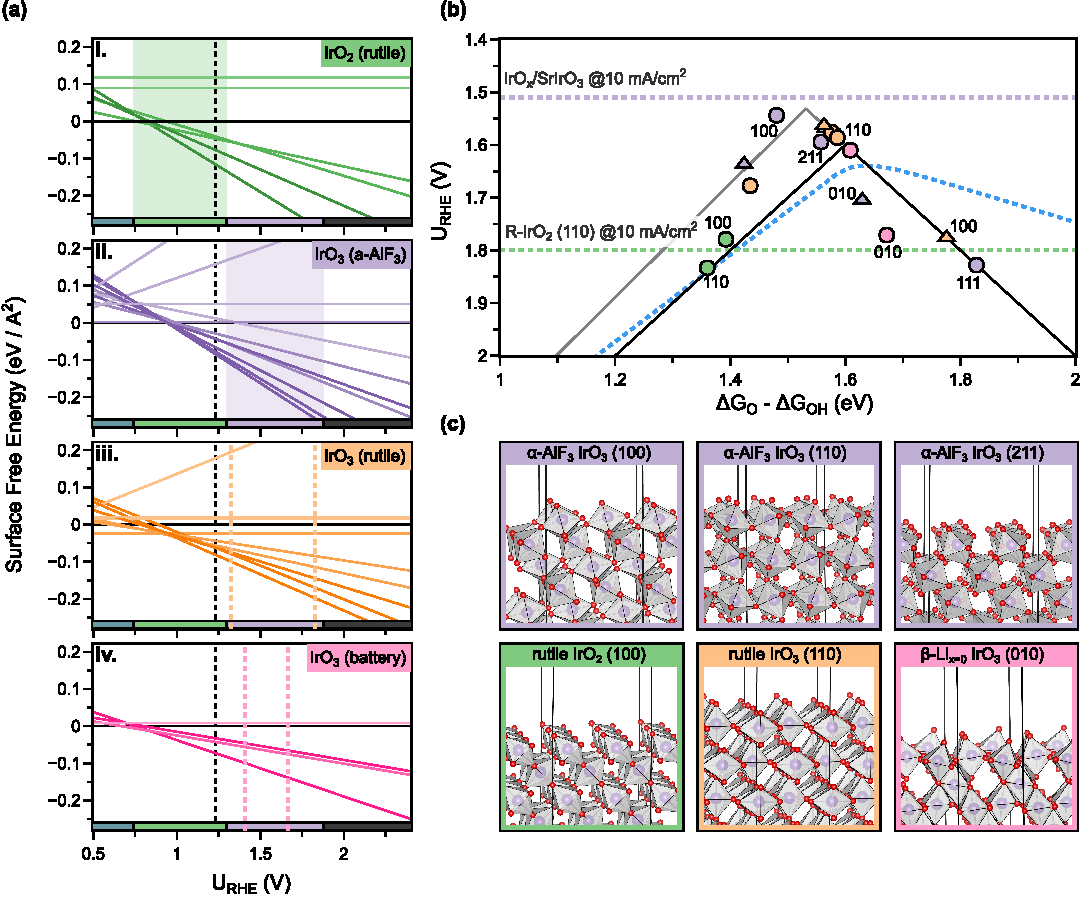
\includegraphics{02_figures/oer_activity_stability/oer_volc_surf_pourb.pdf}}
\caption{\label{fig:oer_volcano}
% TODO Insert green band into figure, insert experimental references for this
%
Summary of OER results for the four bulk structures of \IrOx considered: rutile-\ce{IrO_2} (green), $\alpha$-\ce{IrO_3} (purple), rutile-\ce{IrO_3} (orange), and $\beta$-\ce{IrO_3} (pink).
%
(a) Surface energy Pourbaix diagrams for each structure, with the surface energy of various facets and coverages shown as a function of applied potential.
%
% COMBAK This may not be necessary, too much clutter on plots
The bulk Pourbaix diagram's bounds of stability at pH \num{0} are superimposed at the bottom of each subplot.
%
(b) OER activity volcano for \IrOx systems considered utilizing the \DGOmOH thermodynamic descriptor.
%
The purple dotted line corresponds to the experimental limiting potential at \num{10} mA cm\textsuperscript{-2} for \ce{IrO_3} \cite{Seitz2016},
while the green band corresponds to the range of experimentally observed overpotentials for pristine \ce{IrO_2} catalysts as reported in literature.
%
(c) Select surface facets for the four \IrOx crystal systems considered.
%
Color legend: oxygen (red), purple (iridium), coordination motif (white).
}
\end{figure*}
% __| =====================================================
% =========================================================


% %%%%%%%%%%%%%%%%%%%%%%%%%%%%%%%%%%%%%%%%%%%%%%%%%%%%%%%%%
% | - OER Volcano
% TODO We don't mention new old/new scaling volcanos
% __|
% %%%%%%%%%%%%%%%%%%%%%%%%%%%%%%%%%%%%%%%%%%%%%%%%%%%%%%%%%
% | - PARAGRAPH BODY
%
% Replace G_O and G_OH with my custom macros for consistency
The OER activity (expressed in terms of the limiting potential) for select oxygen terminated surfaces are shown in Figure \ref{fig:oer_volcano}b plotted against the \DGOmOH thermodynamic descriptor.
% $\Delta G_\mathrm{O} - \Delta G_\mathrm{OH}$ 
%
The corresponding surface structures for select systems are visualized in \ref{fig:oer_volcano}c.
%
The \rIrOtwo surfaces bind the OER intermediates relatively strongly,
with theoretical limiting potentials of \mytilde\num{1.8} V vs. RHE (overpotential of 0.57 V vs. RHE) with a *O to *OOH potential limiting step.
%
% Cite Cr-IrO2 paper (ours) and something else here
These results are in agreement with previous experimental, and the lastest theoretical studies.
%
The predicted overpotentials of our \rIrOtwo systems are within the range of experimentally observed overpotentials found in literature.
%
% Reference all experimental IrO2 overpotentials I can find
The surfaces of the three \IrOthree polymorphs have \DGOmOH descriptor values shifted to higher energies, indicative of weaker binding energetics (see \ref{fig:scaling_relations}).
% The three \IrOthree polymorph surfaces all have a $\Delta G_\mathrm{O} - \Delta G_\mathrm{OH}$ descriptor towards the top and right of the volcano, indicative of weaker binding energetics.
%
% COMBAK Report just *OH, I have the other ones to
% O: 1.2 eV; *OOH: 1.4 eV
On average, the binding for *OH is weakened by 0.7 eV relative to \IrOtwo.
%
The highest performing systems include the (100), (110), and (211) facets of \aIrOthree, \bIrOthree (101), and \rIrOthree (110).
%
These surfaces have overpotentials of \mytilde\num{0.4} V vs. RHE,
which represents a \mytilde\num{0.2} V vs. RHE improvement over \rIrOtwo.
%
The primary driver for the improved OER activity is the higher oxidation state of \IrOthree compared to \IrOtwo (+6 and +4, respectively).
%
The comparitively more oxygen saturated \IrOthree systems thus bind OER intermidates more weakly, which for overbinding materials like \IrOtwo and \RhOtwo leads to more ideal scaling.
%
The exact improvement in the theoretical overpotential is slightly dependent on the DFT level of theory and the inclusion of spin polarization, and has been discussed recently.~\cite{Seitz2016,Strickler2019}
%
% TODO COMBAK There should be one more sentence about microkinetic volcano
Additinolly, we include a micro-kinetic volcano for the OER from recent work by Dickens \latin{et al.}~\cite{Dickens2019},
which plots the potential needed to reach a current density of 10 mA/cm2 at a function of the \DGOmOH descriptor.
%
% We note that the computed  overpotentials for our \rIrOtwo system differs from that reported in literature~\cite{Seitz2016} by \mytilde\num{0.2} V.
%
% This discrepancy is due to our inclusion of spin-polarization in our \latin{ab-initio} calculations, which was neglected in Seitz \latin{et al.}.
%
% For further details, we'll refer readers to the SI of a previous publication.\cite{Strickler2019}
% __|
% %%%%%%%%%%%%%%%%%%%%%%%%%%%%%%%%%%%%%%%%%%%%%%%%%%%%%%%%%
